\chapter{Case Study}
\label{case_study_chapter}
Although a thorough evaluation of the developed visual debugging system in general and ROSDashboard in particular was not possible during the course of this work, a case study was conducted to demonstrate the possibilities of such a system. The three cases in this case study show how ROSDashboard can be used with a simple example from the ROS tutorials, how it can be extended with further visualization widgets and how it was used in a real life project to investigate a problem during development.

The first case shows how to connect ROSDashboard's visualization widgets to existing topics in a ROS project. The ROS turtlesim tutorial was chosen as a simple scenario which can be easily reproduced. The example requires no in-depth knowledge of robot programming with ROS since it is created on top of one of the initial tutorials that explain the ROS concepts. The second case in this chapter introduces a new visualization widget for ROSDashboard: The plot widget. This widget can be used to plot data on a Cartesian coordinate system, similar to the dedicated ROS tool rxplot. This case shows how easy it is to extend the current dashboard implementation with further visualization widgets, which was one of the initial requirements for the visual debugging system designed in Chapter~\ref{visual_debugging_system}. The last case examines the use of ROSDashboard during the development of a real life robotics project. An existing problem that appeared during the development of a robotic system with the NAO humanoid robot was investigated using ROSDashboard.

\section{Simple ROSDashboard Example}
Figure~\ref{showcase} shows a simple example how ROSDashboard can be used during development. ROSDashboard is running alongside the \emph{turtlesim\_node} node which is used in many examples in the ROS tutorials\footnote{\url{http://www.ros.org/wiki/ROS/Tutorials}}. It monitors the values for linear and angular speed which are published by the \emph{turtle\_teleop\_key} node to control the turtle simulation. The String widget is configured to display logging messages published on the \emph{/rosout} topic, which in this example shows a warning when the turtle hits a wall. For the purpose of this simple example, there was no need to modify the turtlesim source code. The only topics used by this scenario are topics that are already used to control the turtle in the simulation and to display warnings.

\begin{figure}[thpb]
  \centering
  \framebox{
    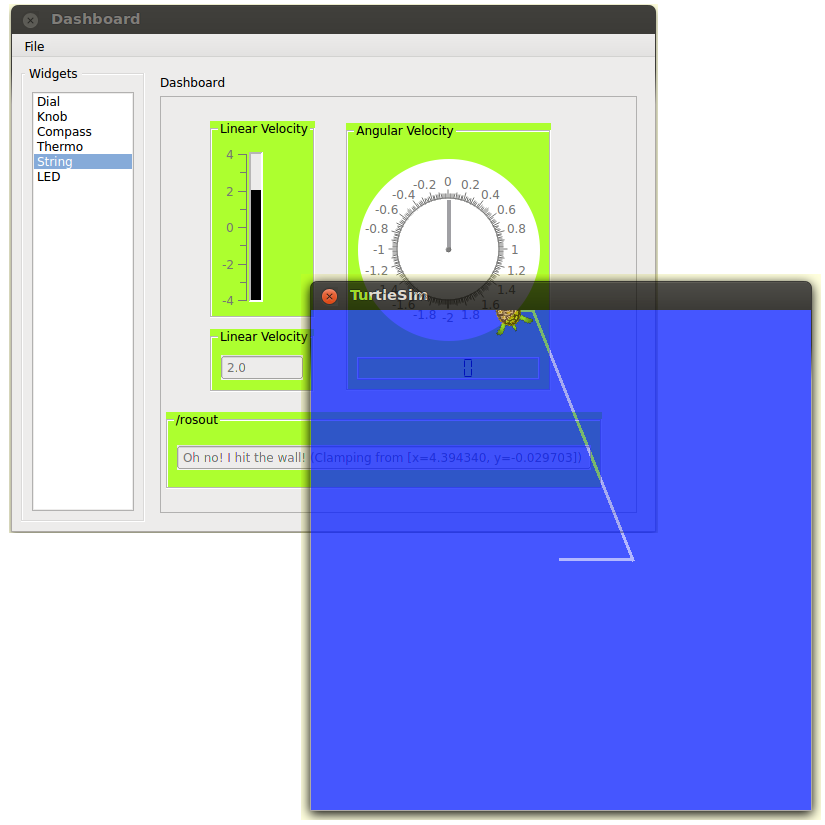
\includegraphics[width=0.9\textwidth]{img/showcase3.png}
  }  
  \caption{ROSDashboard running alongside turtlesim\_node.}
  \label{showcase}
\end{figure}

The ROS computation graph during the execution of this scenario is shown in Figure~\ref{rosgraph_simple}. It shows how ROSDashboard is connected to the nodes which are debugged. The topics needed for the example are \emph{/turtle1/command\_velocity} for the linear and angular velocity and \emph{/rosout} for warnings when the turtle hit the wall.

\begin{figure}[thpb]
  \centering
  \framebox{
    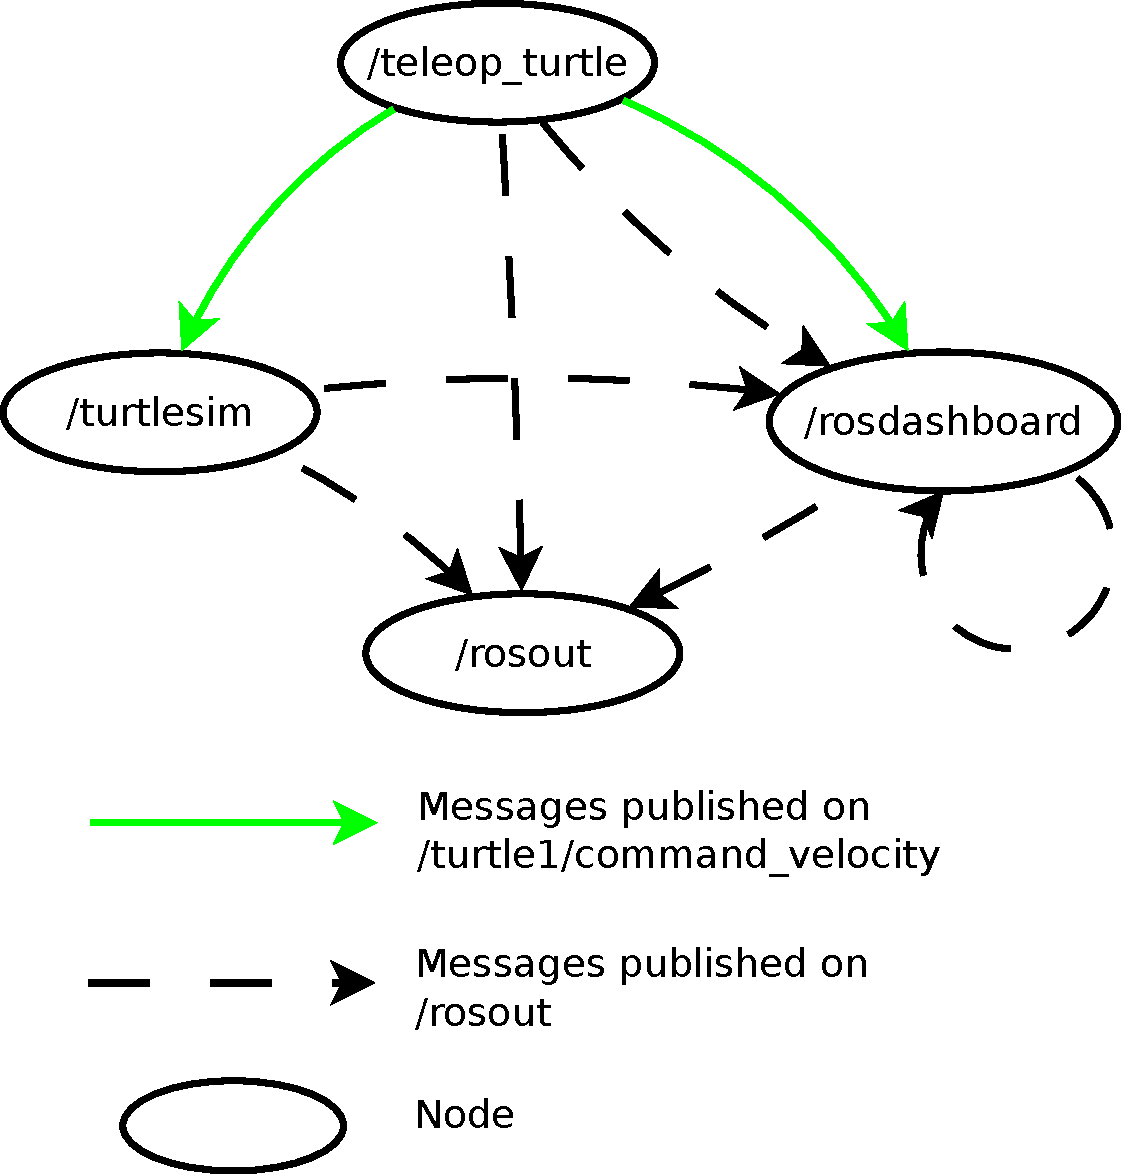
\includegraphics[width=0.7\textwidth]{diagrams/rosgraph}
  }  
  \caption{Simplified ROS computation graph with ROSDashboard.}
  \label{rosgraph_simple}
\end{figure}

\section{Adding a New Widget}
\label{plot_widget_section}
\begin{figure}[htb]
  \centering
  \framebox{
    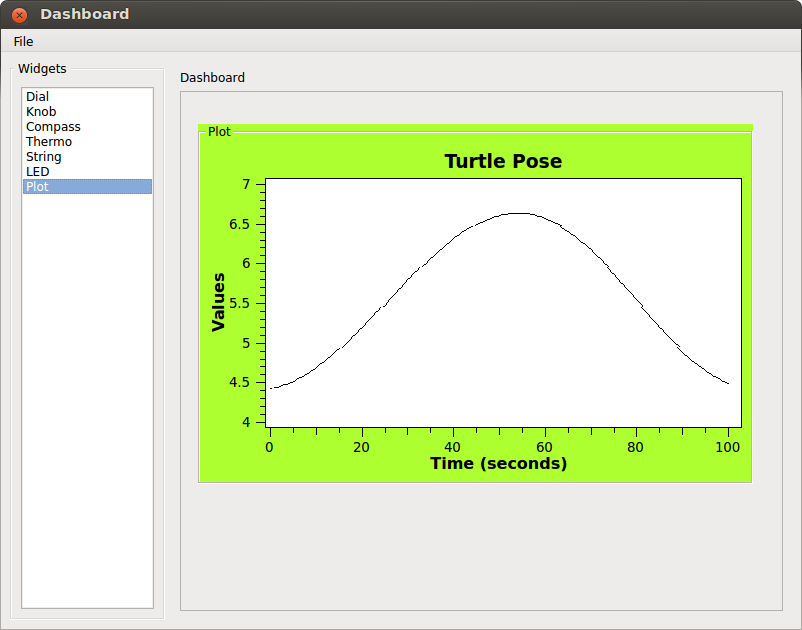
\includegraphics[width=0.9\textwidth]{img/plot_widget.png}
  }  
  \caption{The newly created plot widget in action.}
  \label{plot_widget}
\end{figure}

Adding new visualization widgets to ROSDashboard is easy. The abstract \textbf{DashboardWidget} class (see Figure~\ref{class overview}) handles most of the generic things a widget should implement. As part of a first evaluation step a new visualization widget was added to the dashboard: A plot widget that plots values on a Cartesian coordinate system. Figure~\ref{plot_widget} shows a screenshot of the new visualization widget in action and the full implementation is appended in Listing~\ref{drag_plot_implementation}.

To implement the widget, a new class called \textbf{DragPlot} was created. The class inherits the basic implementation from \textbf{DashboardWidget} and only needs to implement the plot specific methods. Upon initialization of \textbf{DragPlot} the user interface part of the widget is created. The class implements the two abstract methods \verb+updateValue+ and \verb+initProperties+ from \textbf{DashboardWidget}. \verb+updateValue+ updates the graphical part of the widget and \verb+initProperties+ adds two properties to the widget: plot name and update rate in milliseconds. This requires only two lines of code, see Listing~\ref{init_props}.

\begin{lstlisting}[float,frame=single,caption={Implementation of initProperties in DragPlot.},label=init_props,language=Python,numbers=left,breaklines=true]
# property keys
TITLE = 'Plot title'
RATE = 'Refresh rate (ms)'

def initProperties(self):
  self.props[self.TITLE] = WidgetProperty('text', 'Plot title')
  self.props[self.RATE] = WidgetProperty('numeric', 500)
\end{lstlisting}

The default implementation in \textbf{DashboardWidget} is capable of automatically generating a user interface for those simple properties. When the properties are updated in the properties dialog, a callback is used to notify the \textbf{DragPlot} class. The callback implementation to update the widget is shown in Listing~\ref{prop_callback}. It updates the title of the plot and starts a new timer which updates the plot in a given interval.

\begin{lstlisting}[float,frame=single,caption={Implemented updateWidget callback in DragPlot.},label=prop_callback,language=Python,numbers=left,breaklines=true]
def updateWidget(self):
  #update the widget properties
  self.qwtPlot.setTitle(self.props[self.TITLE].value)

  if (self.currentTimerId != 0):
    self.qwtPlot.killTimer(self.currentTimerId)
    self.currentTimerId = 0

  self.currentTimerId = self.qwtPlot.startTimer(self.props[self.RATE].value)
\end{lstlisting}

The plot itself is a \textbf{QwtPlot} widget from the popular QWT widget library\footnote{\url{http://qwt.sourceforge.net/}}. To customize the plot widget, \textbf{QwtPlot} was subclassed in \textbf{DataPlot}. The \textbf{DataPlot} class exposes two methods: \verb+addValue(value)+ and \verb+timerEvent()+. The \verb+addValue(value)+ method is used in the implemented abstract method \verb+updateValue(value)+ from \textbf{DashboardWidget} and adds a new value to the plot. \verb+timerEvent()+ is a callback that gets triggered regularly, how often depends on the update rate which can be set in the properties of the widget.

The last step to add the new visualization widget to ROSDashboard is to add it manually to the list of available visualization widgets which appears in the toolbox left of the dashboard canvas. This example shows how easy it is to add a new widget to ROSDashboard. A plugin architecture would make it even easier, since the last manual step is not required and widgets could be dynamically loaded as plugins.

\section{Real Life Project}
\label{nao_case}
A recent problem during the development of an existing project was chosen to show how ROSDashboard can be used for debugging in a real life project. The project's goal is to use the NAO humanoid robot together with ROS to follow people and engage in conversations with them.

The NAO is a humanoid robot developed and sold by Aldebaran-Robotics\footnote{\url{http://www.aldebaran-robotics.com/}} \cite{Gouaillier2008}. Figure~\ref{nao_coffee} shows an image of the NAO robot used during this experiment. The robot comes with a comprehensive list of high level software modules that can be used: a text-to-speech module, a voice recognition module, a walking engine, sound localization, etc. Developers also have access to low level sensor information and can control the actuators directly. The robot is shipped with Choreographe, a graphical programming interface to combine the high level modules to behaviours and create new behaviours from scratch.

\begin{figure}[htpb]
  \centering
  \framebox{
    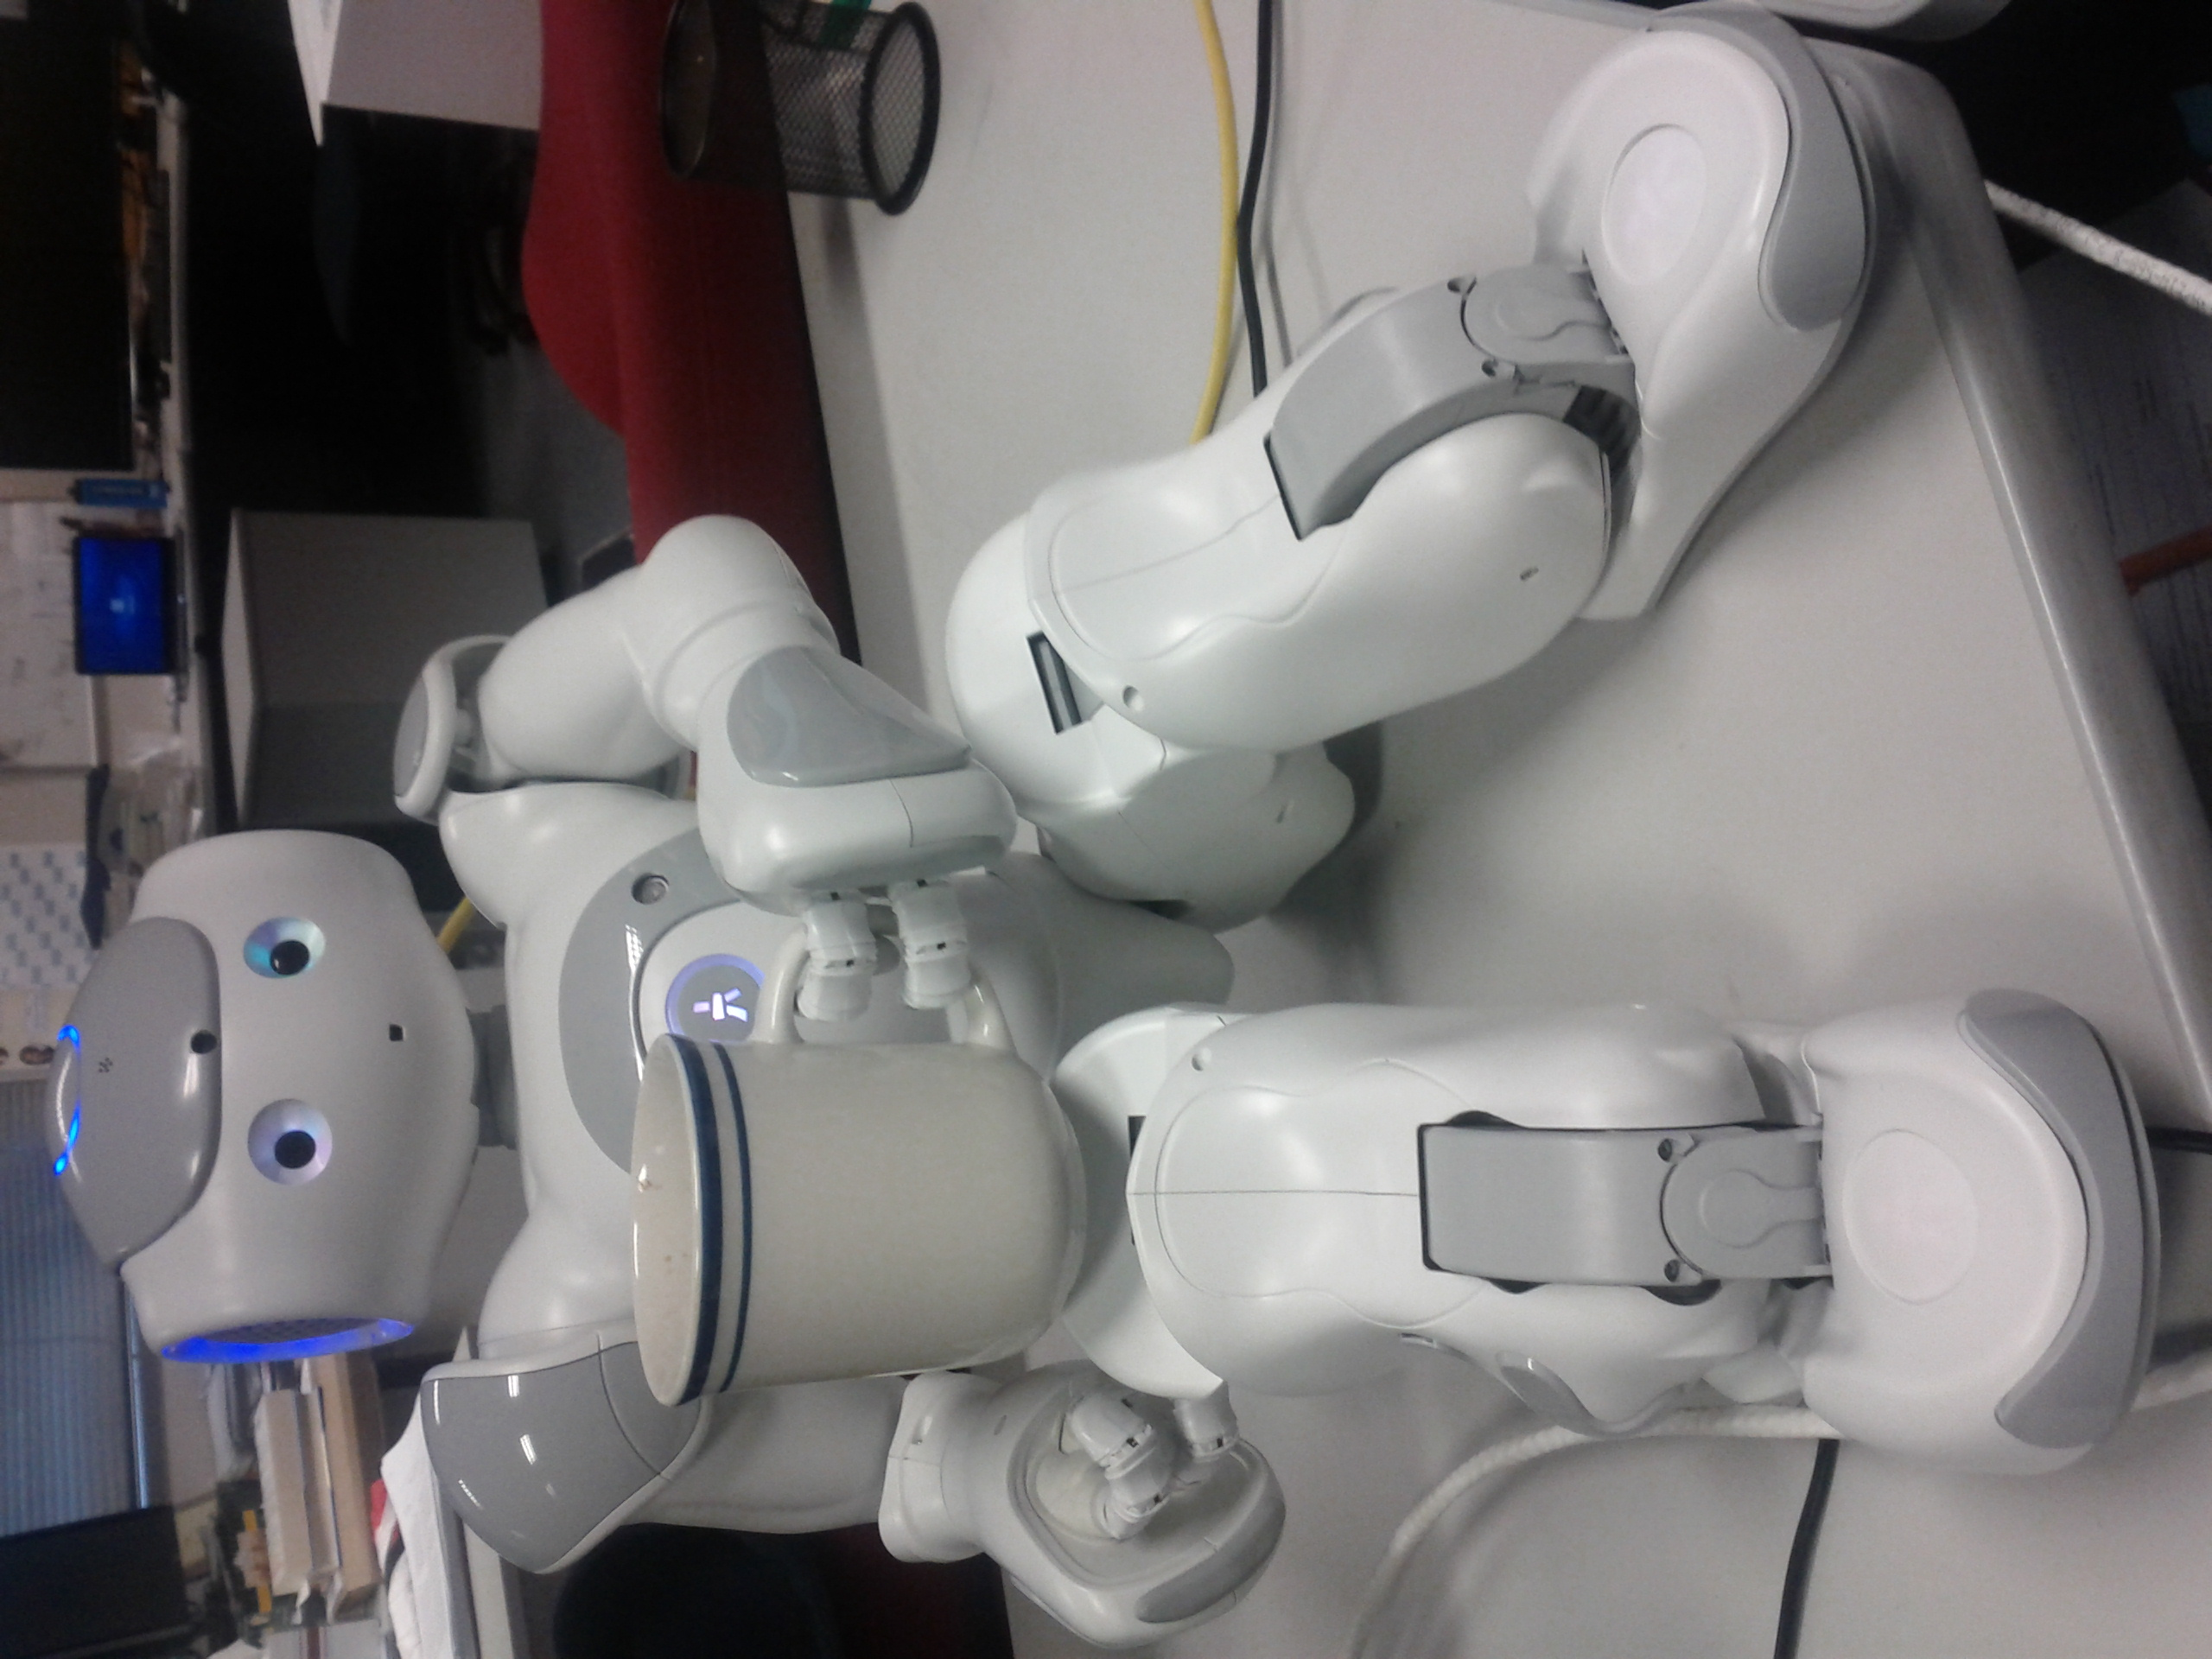
\includegraphics[angle=270,width=0.4\textwidth]{img/nao_coffee.jpg}
  }  
  \caption{NAO robot during the experiment.}
  \label{nao_coffee}
\end{figure}

In the project targeted for this experiment the sound localization module was used to move the head towards the person talking to the NAO robot. The sound localization algorithm is part of the SDK and can be accessed through the robot drivers in ROS, which publish the estimated position of a sound source to a topic. The algorithm publishes the location where the sound comes from as a triplet of the horizontal location (azimuth), vertical location (elevation) and confidence. During the initial experiments with the ``Sound Tracker'' module in Choreographe it seemed like the NAO robot would sometimes point the head to a random direction unrelated to the real direction of the sound source.

The developer of this system tried to find out whether the problem lies with the accuracy of the sensor, the implementation of the sound localization algorithm or the ``Sound Tracker'' module moving the head. Since the data from the sound source is published as a triplet of numbers, debugging the issue by looking at numbers in a console was challenging. ROSDashboard was used to visualize the values from the sound localization algorithm to determine where the problem of wrong head positions originated.

This section first presents the experimental setup for the tests with the NAO robot. The second part explains how the experiment was conducted with the NAO robot and ROSDashboard, which leads to the results in the third part of this section.

\subsection{Experiment Configuration}
The setup during this experiment was distributed on three different machines. The NAO robot runs on a built in Linux which communicated with the master node where the ROS core, Choreographe and the NAO drivers were running. The third machine was a laptop running ROSDashboard and connecting to the respective ROS topics over the network. All three machines were connected to a router by cable. The master node and the laptop with ROSDashboard were both running with Ubuntu 12.04 (64bit) and had ROS Fuerte, the latest ROS release installed.

While the robot was operated directly by Choreographe, a ROS node was executed as part of the NAO drivers for ROS which published the three values from the sound localization algorithm on the \emph{/sound\_source} topic. The data from this topic was visualized in ROSDashboard. A compass widget was used to visualize the azimuth value from the localization algorithm which represents the horizontal location of the sound source. Since the data published by the localization algorithm is in radiants, it first had to be transformed into degrees for better visualization. Apart from the compass widget a dial was used to visualize the raw radiant value from the algorithm and a thermo widget was used to visualize the confidence as a vertical bar ranging from zero to one. Figure~\ref{nao_dashboard_screenshot} shows the configuration of widgets during the experiment, which is also available in its JSON representation in Listing~\ref{nao_dashboard_file} in the appendix.

\begin{figure}[htpb]
  \centering
  \framebox{
    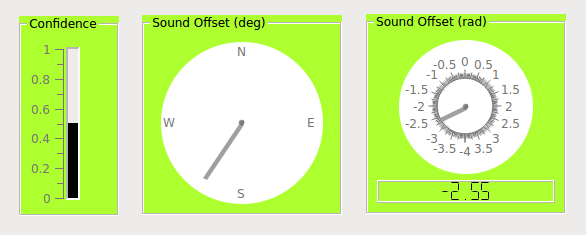
\includegraphics[width=0.9\textwidth]{img/nao_dashboard_screenshot.png}
  }  
  \caption{Widget configuration during the NAO experiment.}
  \label{nao_dashboard_screenshot}
\end{figure}

\subsection{Experiment}
A series of tests were conducted to understand what the values from the sound localization algorithm meant. Several sound sources were created by clapping in close proximity to the NAO robot or simply by talking towards the robot. The first set of test were done with an activated ``Sound Tracker'' module in Choreographe, which in result moved the head immediately once the NAO robot detected a sound source with a confidence level above a certain threshold. The second set of test was conducted without the ``Sound Tracker'' module and thus with a static head fixed to its origin. First visualizations of the azimuth value were misleading, but during the experiment it became obvious that the position of the sound source is calculated relative to the position of the head and not relative to the position of the body of the robot which was not moving while the tests were performed. Further research explained this observation, since the microphones used to determine the location of the sound source are all positioned on the head of the NAO robot.

The tests performed during the experiment also showed that the sound localization algorithm usually detects the location of the sound source correctly, but while the head is moving to the desired position more readings come in from the algorithm. These estimated positions were most of the time less confident than the initial sound localization. If the threshold to move the head was set too low, the robot was interrupted during the movement of the head to the position estimated at first and moved the head to a different position. This made the head movement seem random and not related to the actual source of the sound, which was the original problem examined in this experiment.

\subsection{Results}
This experiment described in this section is based on an existing problem that happened during the development of a small but real life robotics project. ROSDashboard was successfully used to visualize data and helped to understand the data published by the sound localization algorithm. In general it also contributed to a better understanding of the robot under development. The data published by the localization algorithm is much easier to interpret and understand using ROSDashoard than looking at the numbers scrolling down in a console. Figure~\ref{comparison} shows the dashboard interface visualizing the data and the raw output printed in a console with the command line tool \verb+'rostopic echo /sound_source'+.

\begin{figure}[ht]
\centering
\subfigure[ROSDashboard]{
    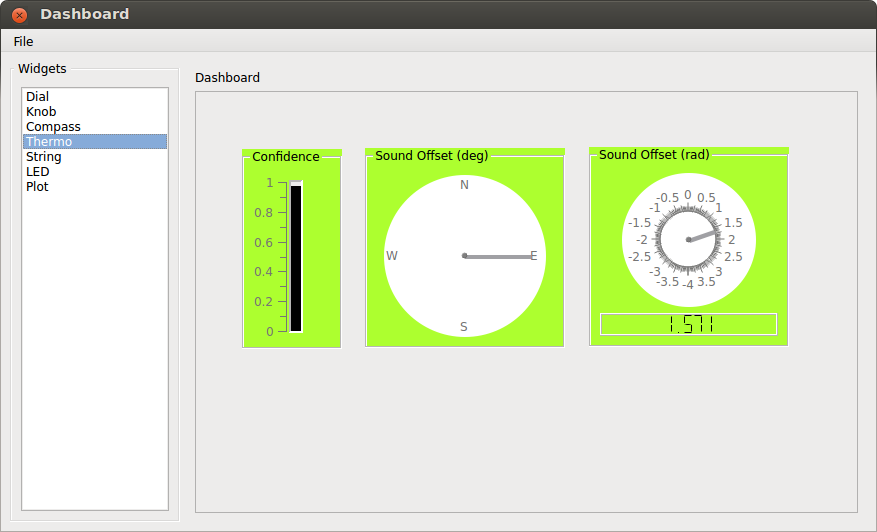
\includegraphics[width=0.9\textwidth]{img/nao_experiment_rosdashboard.png}
}
\subfigure[Console]{
    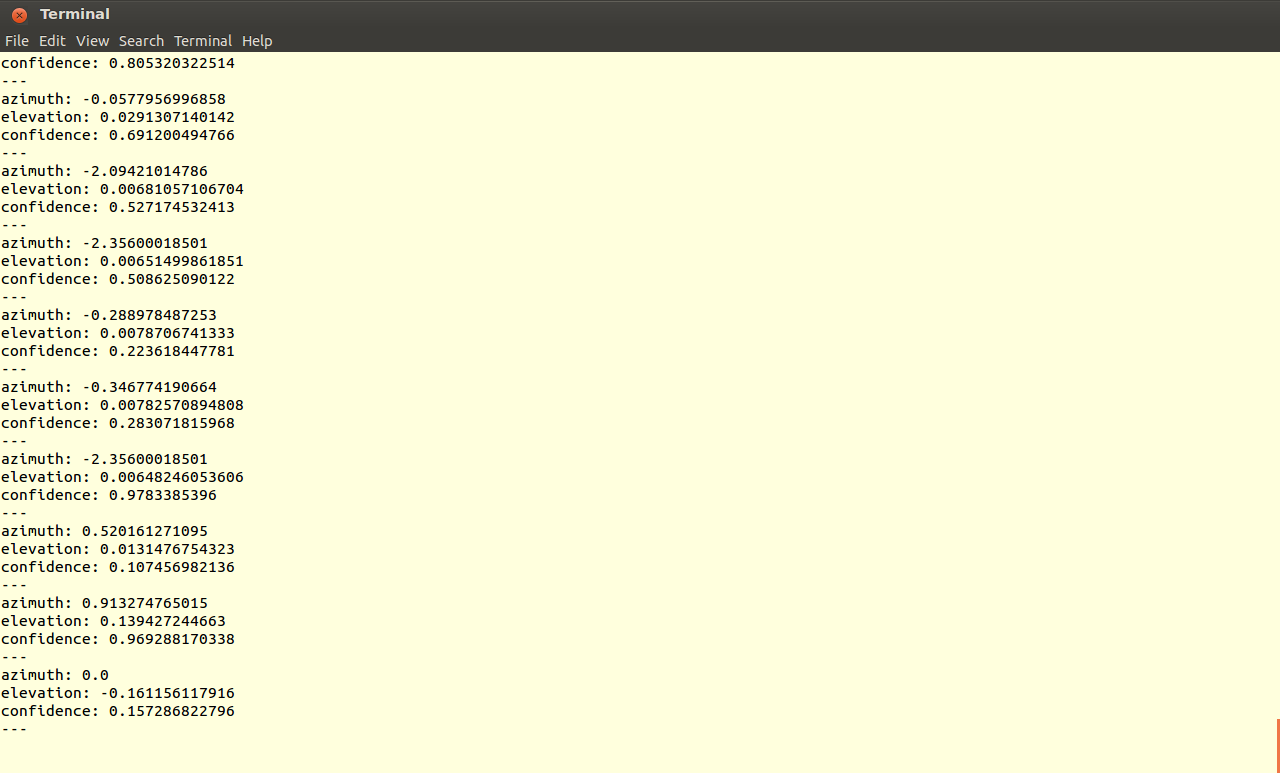
\includegraphics[width=0.9\textwidth]{img/nao_experiment_console.png}
}
\caption{Side by side comparison of ROSDashboard and console output during the experiment.}
\label{comparison}
\end{figure}
